\documentclass[utf8]{frontiersinFPHY_FAMS}
\setcitestyle{square}
\usepackage{url,hyperref,lineno,microtype,subcaption}
\usepackage[onehalfspacing]{setspace}
\linenumbers
\def\keyFont{\fontsize{8}{11}\helveticabold }
\def\firstAuthorLast{Bagby-Wright {et~al.}}
\def\Authors{Christian Bagby-Wright\,$^{1,*}$, Daniel Welling\,$^{2}$ and Roxanne Katus\,$^{3}$, Brian Walsh\,$^{4}$}
\def\Address{$^{1}$University of Texas at Arlington, College of Science, Department of Physics, Arlington, TX, USA \\
$^{2}$University of Michigan, College of Engineering, Climate and Space Sciences and Engineering, Ann Arbor, MI, USA  \\
$^{3}$University of East Michigan, College of Arts and Sciences, Mathematics and Statistics, Ypsilanti, MI, USA \\
$^{4}$Boston University, College of Engineering, Department of Mechanical Engineering, Boston, MA, USA}
\def\corrAuthor{Christian Bagby-Wright}

\def\corrEmail{christian-an.bagby-wright@mavs.uta.edu}

%\newcommand{\note{}}[1][0]{\color{red}{} \color{black}}
%\newcommand{\Re}[1][0]{$R_{E}$}
%\newcommand{\BATS}[1][0]{Block-Adaptive-Tree-Solar-Roe-Up-Wind-Scheme }
%\newcommand{\bats}[2][0]{BATS-R-US }
%\newcommand{\DGCPM}[3][0]{Dynamic Global Core Plasma Model }
%\newcommand{\dgcpm}[4][0]{DGCPM }
%\newcommand{\SWMF}[5][0]{Space Weather Modeling Framework }



\begin{document}
\onecolumn
\firstpage{1}
\title[Recirculation of the Plasmasphere]{Recirculation of Plasmasphere Material During Idealized Magnetic Storms} 
\author[\firstAuthorLast ]{\Authors} %This field will be automatically populated
\address{} %This field will be automatically populated
\correspondance{} %This field will be automatically populated
\extraAuth{}
\maketitle
\begin{abstract}

%%% Leave the Abstract empty if your article does not require one, please see the Summary Table for full details.
%The abstract should be succinct, while rendering the general significance and conceptual advance of the work clearly to a broad readership. Don't cite References in Abstract. 
\section{}

The fate of flux tube material once it is drained out of the plasmasphere through a day side plume has been unknown for a long time. One of a few things can happen to the vented plasmasphere material. It can be either swept away by the solar wind and lost to the earth system, be injected into the ionosphere, %I'm not really sure about this part. Dr. Deng asked about it and while flow vectors in the sim don't suggest it, I don't have as strong a reason as I would like to deny this. The particles in the plasmasphere presumably didn't have the pitch angle to be in the loss cone, and so would fall into the ionosphere, however it possible that the changing lambda of the B-field foot point combined with energerzation from the recirculation process would change the pitch angle. Need to play with the equations a bit to see if it's practical 
or recirculate into the magnetosphere system. Recirculating plasmasphere material could plausibly enter the central plasma sheet and contribute to the ring current. This work uses numerical models to answer this question. Historically this has been a difficult question to answer due to the fact that solar wind, ionosphere, and plasmasphere plasmas are all dominated by hydrogen making it difficult to distinguish the source of plasma from observation alone. Recent advances in computing however have enabled us to answer this question. Using the Space Weather Modeling Framework (SWMF) to couple together the Block-Adaptive-Tree-Solar-Roe-Up-Wind-Scheme (BATS-R-US), Dynamic Global Core Plasma Model (DGCPM), and the Ridley Ionosphere Model (RIM), we can track the motion of the plasmasphere material once it leaves the plasmasphere in a novel self-consistent manner. %Rewrite that sentience.

\tiny
 \keyFont{ \section{Keywords:} plasmasphere, recirculation, inner magnetosphere, simulation, reconnection} %All article types: you may provide up to 8 keywords; at least 5 are mandatory.
\end{abstract}

\section{Introduction}

%Keep it succinct. No subheadings!
The plasmasphere is a cold ($\sim1$ eV) dense ($10^{3}-10^{4}$) region of plasma which corotates with Earth. The plasma in the plasmasphere has primarily large pitch-angles and so is confined mostly to the equatorial plane. During extended periods of low activity in the solar wind, the plasmasphere fills up to a saturation density as it reaches a diffusive equilibrium with the ionosphere. During periods of high activity, enhanced dayside reconnection with the Interplanetary Magnetic Field (IMF) causes mass-loaded magnetic flux tubes in the plasmasphere to be advected out to the reconnection region as described by the \citet[Dungey(1961)]{dungey1961interplanetary} during southward interplanetary magnetic field. %The journal states to write the abstract (and I assume the article) for a board audience should I take the time to explain magnetic reconnection and the Dungey cycle?)
As the process of magnetic reconnection continues along the dayside magnetopause, a plume of material forms on the dayside, draining plasma from the plasmasphere along the path of the advecting  %find a better word? Is this a confusing phasing. 
 flux tubes. The plasma remains trapped on the field line through the process of reconnection and remains with the field line as it continues through the Dungey cycle. At this point, the field line is no longer closed with both ends on Earth, but is rather an open field line, with one end anchored to Earth and the other connected to the IMF. The question at this point is if the velocity of the trapped plasma along the the field line is large enough that a significant fraction of it is within the loss cone, to be lost to scattering in the ionosphere, or travel further into the IMF before being trapped by reconnection on the night side. The plasma could recirculate through one of two paths.  The first is that the plasma can be transported through the lobes by the advecting magnetic flux tubes and become trapped on closed field lines due to magnetic reconnection on the night side. Alternatively the plasma could recirculate by traveling along the flanks and mixing with the plasma sheet material in the tail through viscous interactions. 

\citet[Borovsky et al.(1997)]{Borovsky1997}, while studying the super dense plasma sheet,demonstrated that plasmasphere material did stay on the field lines as they underwent reconnection, having bulk flow velocities to remain on the now open field lines. The study made use of satellite data from ISSE 3, several LANL spacecraft at geosynchronous orbit, and the OMNI data set. While this was sufficient to show that plasmasphere material stayed with its magnetic field lines just after magnetic reconnection, the nature of the satellite orbits and on board instruments meant that he could not trace the material through any path that might lead to recirculation. Furthermore, the homogeneous nature of the plasmasphere and solar wind composition makes it difficult for a satellite mission to distinguish which population was the source of detected plasma. Despite these limitations Borovsky estimated that the recirculating plasmaspheric material should predominately be recaptured on the night side given its low velocity along the magnetic field line at the last point of measurement. 

If plasmasphere material did recirculate it would enter the plasma sheet, where it might contribute to the ring current. Ring current ions primarily come from the plasma sheet and the solar wind. However, the plasma sheet is itself fed by the ionosphere and the solar wind. Thus, the ultimate source of ring current particles is the ionosphere and solar wind \citet[Daglis et al.(1999)]{Daglis1999}. %this citation behaving weird
This leaves us with a contradiction, \citet{Borovsky1997} estimates that the plasmaspheric plasma should recirculate and be returned up the magnetotail, yet  \citet{Daglis1999} argues that the plasmasphere is not a significant contributor to the ring current based on composition and charge state observations of the ring current. %I'm not sure if the preceding sentence is entirely clear. It gets the point across but I might be overstating both authors cases and the statements they make. 
 The question of the fate of the plasmasphere material once it enters the solar wind, has remained open since that time, due in part to the difficulty in answering it. 

Using observations to resolve the issue is difficult due to the homogeneous nature of the plasma from the solar wind, plasmasphere, and ionosphere, which are all dominated by hydrogen. For some time simulations have not been up to the task of tracking multiple populations of ions in the magnetosphere on a global scale, due both to a lack of computational power and the short outer boundary of dedicated plasmasphere codes not being large enough to capture recirculation.  However, recent advancements both in modeling approaches and computing power have made it possible to study the fate of the plasmasphere in numerical simulations. 

This study presents four simulations using the Space Weather Modeling Framework in a novel configuration to study the fate of plasmaspheric material during magnetic storms. The simulations approach the recursive relationship of the inner magnetosphere and solar wind coupling from a self-consistent manner. This will enable us to address the fate of the plasmasphere once it enters to solar wind, and begin to resolve the outstanding question. 

\section{Methodology}
\subsection{Configuration of the SWMF} %I'm being purposefully obtuse with 'spacio-chronatic', I'm having fun while writing. 
It is difficult to design a model which captures the intricacies of the near-earth space environment due to the large change in spacio-chronatic scales, composition, and physics. The Space Weather Modeling Framework \citet[Toth et al.(2005)]{Toth2005} accomplishes this goal by coupling together models which are specialized to capture the dynamics of sub regions, or particular processes, of space weather. This coupling typically includes passing information about key values, such as density and temperature of a plasma, between models to ensure that they are in sync both temporally and spatially in regards to key parameters. For this study the SWMF is configured to couple three models. The Block-Adaptive-Tree-Solar-Roe-Up-Wind-Scheme (BATS-R-US), the Dynamic Global Core Plasma Model (DGCPM), and the Ridley Ionosphere Model (RIM). BATS-R-US is a global magnetohydrodynamic code configured with two fluids, both hydrogen. The first fluid is defined to be the known sources of the ring current namely the solar wind and the high latitude ionospheric outflow (I will refer to this fluid as sw). The second BATS-R-US fluid is the plasmasphere coupled to DGCPM (I will refer to this fluid as iono). DGCPM is a two dimensional code which solves for flux tube content on the ionosphere grid, projected into the equatorial plane. DGCPM is configured within the Space Weather Modeling Framework to have one way coupling with BATS-R-US in which dynamics on closed field lines within $10 R_{E}$ are determined by DGCPM which overwrites BATS-R-US's own solution within that region. BATS-R-US is coupled to RIM in a two way manner, passing field aligned current information to it while receiving the electric field. RIM and DGCPM are one way coupled, where DGCPM uses the solution of the electric field generated by RIM as its inner boundary condition rather then an embedded empirical model. For a graphical representation of this configuration refer to figure \ref{fig:Configuration}.

\begin{figure}[!ht]
\begin{center}
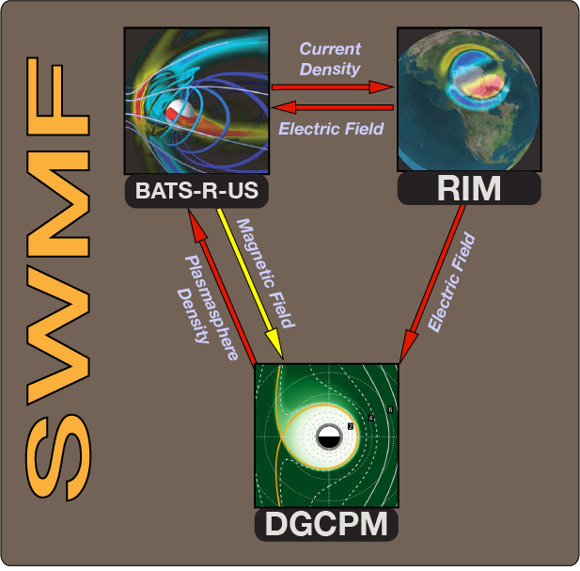
\includegraphics[width=0.5\textwidth]{SWMF_config.png}
\caption{Configuration of the SWMF and coupling between sub modules}
\label{fig:Configuration}
\end{center}
\end{figure}


Several simplifying assumptions were made in this simulation. First is that the earth's magnetic field could be represented as a dipole, second that the dipole pointed along the earth's axis of rotation, and third that the axis of rotation is perpendicular to the ecliptic plane. SWMF runs on a Cartesian grid with the positive x-axis pointing from the center of the earth to the sun, the positive z-axis pointing along the earth's axis of rotation, and the positive y-axis pointing from the center of the earth to dusk local time, completing the right-handed coordinate system. The SWMF runs in two portions, a steady state portion and a time accurate portion. The steady state portion is used to create a more realistic magnetic field from the initial conditions then the truly ideal start point. The steady state portion ran for 5000 iterations, during which it adjusted the magnetic field and refined the grid of BATS-R-US.

\subsubsection{Configuration of BATS-R-US}
%how do I cite the SWMF manuel? 

BATS-R-US is a multi-fluid multi-species global magnetohydrodynamic code. It handles the bulk of the computational space while the other models, DGCPM and RIM, handle specific components of the inner magnetosphere and ionosphere. A key feature of BATS-R-US is the dynamically selected grid size of cells within the region of computation. The size of a grid cell in BATS-R-US depends on the initial grid defined by the user and refinement that happens during the simulation. Periodically the simulation will pause to refine the grid, adding resolution to areas with high local wave speeds and fluid densities, and removing it from areas with low values. This enables BATS-R-US to capture dynamics regardless of where in the computational domain they may occur with out wasting time on computing mostly empty space far from regions of interest.

 For our simulations the maximum size of a single cubic cell in the computational domain is 8 Earth Radii ($R_{E}$) while the finest resolution is $1/16 R_{E}$. Initially the grid is set with areas of high resolution around the earth, stepping down from $1/16 R_{E}$ cubic cells nearest the earth to cells of $1 R_{E}$ furthest from the earth. The steady state portion additionally refined the grid from the initial layout every 100 iterations. After the refinement areas of high resolution are primarily around the magneto pause (sheath?), and polar lobes while regions far down tail lose resolution. For a more detailed discussion of the grid see \citet[Welling and Liemohn(2014)]{Welling2014}.

Within BATS-R-US the upstream boundary condition is determined by solar wind and interplanetary magnetic field (IMF) values read from a file. In addition to the IMF field and solar wind conditions, values must be provided for every fluid in the MHD simulation. This is because the numerical schemes of BATS-R-US cannot handle zero densities or temperatures and must have all the ions present in the whole computational domain. As such low values are chosen for non-dominant ions such that their contribution to total density and energies are negligible in the region dominated by the solar wind. The inner boundary is determined by predefined values made to mimic the polar wind, specifically in the MHD simulation it was set to 28 amu/cc at 25000.0 $^{\circ}$K for sw, the fluid representing the combined solar and polar wind. Similar to the upstream requirements both fluids of the MHD simulation require an inner boundary value. For the iono fluid, values of .01 amu/cc and 25000 $^{\circ}$K were assigned. The low amu/cc count of iono prevents the inner boundary condition of iono to become a significant source of plasmasphere ions. 

%Don't go into every little detail of the PARAM file, hit the high points then tell them to reference supplements. 

%The first thousand iterations of the steady state simulation uses a first order Rusanov scheme, while the remainder of the simulation uses a second order Rusanov solver. The first order Rusanov scheme users a one-stage time integration, while the second order scheme makes use of 

%The equation of state in BATS-R-US are set to be non-conservative. The pressure equation is solved and from this the total energy density is calculated, using the pressure, kinetic and magnetic energy densities in the region defined by a parabola $(y**2+z**2) /15$ whose value is x = 5 or less. %Ask for clarification of what the conservative criteria command means
%Outside this region a conservative scheme is applied. In the conservative scheme the total energy equation is solved everywhere and the pressure is derived from this value. 

Ion-Ion collisions are neglected. The equations of state are non-conservative within a parabola described by $(y**2+z**2) /15$ whose value is x = 5 or less. %pretty sure this broadly mirrors the magnetosheath. 
In the non-conservative method the pressure density equation is solved and that is used to calculate the total energy density, outside of this region the total energy density equations are solved. 

\subsubsection{Configuration of DGCPM}

DGCPM is a single species semiempirical two-dimensional code solving for the flux tube content measured in electrons per Weber \citet[Jorgensen et al.(2017)]{Jorgensen2017}. In the filling and emptying of dayside, closed magnetic field lines, DGCPM works to drive each flux tube towards its saturation density. The saturation density was determined empirically by Carpenter and Anderson(1992) as, %\citet[Carpenter and Anderson(1992)]{Carpenter1992}. get reference when internet come back online

\begin{equation}
	n_{sat} = 10^{(-0.3245L+3.9043)}
	\label{eq:METH1}
\end{equation}

given in electrons per cubic centimeter, where L is the L-shell of the field line in the equatorial plane. On the day side closed flux tubes whose density exceed $n_{sat}$, have their density reduced to the saturation value. If however the density on such a field line is less then $n_{sat}$ a refilling flux is applied, up to a pre-defined maximum flux. On open field lines, night or day, the same decay rate is applied. A decay rate is also applied to closed field lines on the night side. For a more detailed discussion on how DGCPM functions see \citet[Ober et al.(1997)]{Ober1997}. % For a discussion on How DGCPM functions as a subset of the SWMF see "That reference doesn't exist"

The temperature of the plasma is fixed to be 2 eV for the purpose of coupling to BATS-R-US, where the temperature and density of the plasma in DGCPM is used to calculate the pressure of the iono in BATS-R-US. DGCPM assumes a dipole field, and does not couple its magnetic field to BATS-R-US. Because BATS-R-US also assumes an ideal magnetic field this causes a minimal difference between the models despite the lack of a coupling between the magnetic fields. %wait, this says that we don't couple the magnetic field, but the graphic says we do. Which is it? This is also a two sentence paragraph. Add more, is just one ok?

The truly novel part of this configuration of the SWMF is that, on closed field lines within 10 $R_{E}$, the dynamics of the plasmasphere fluid in BATS-R-US are dictated by DGCPM. By doing so we get a far more realistic plasmasphere then what a MHD code could produce on its own. Seen in fig \ref{fig:METH1} is a comparison of the plasmapshere in different configurations of BATS-R-US and DGCPM. In \ref{fig:METH1}a we see the plasmasphere as produced by BATS-R-US running in a stand alone single fluid configuration. In \ref{fig:METH1}b is BATS-R-US in a multi-fluid stand alone configuration, with a dedicated plasmasphere fluid. \ref{fig:METH1}c Is a stand-alone DGCPM simulation, while \ref{fig:METH1}d is a coupled multi-fluid BATS-R-US and DGCPM running as subcomponents of the SWMF. As can be clearly seen in \ref{fig:METH1}a and \ref{fig:METH1}b a global magnetohydrodynamic code, even with a dedicated plasmasphere fluid, is a poor representation of the dynamics a cold dense plasma undergoes near the earth. The stand-alone DGCPM simulation gives a very detailed plasmasphere, but lacks the ability to model the solar wind, plasma sheet, and anything beyond 10 $R_{E}$ of the earth. While this gives us a detailed view of the population in question it limits our understanding of the entire system. Thus, by coupling DGCPM to BATS-R3-US we capture the best of both worlds, able to see and model the solar wind, and the broader near earth space environment, while maintaining a detailed view of the plasmasphere. Most importantly this enables us to study in a self-consistent manner how plasmapshere material evolves once it enters the solar wind, and whether or not it is captured by night side reconnection and advected back towards the earth. 

%I'll need to get another version of this file as I need one with labeled subplots as per Frontiers requirements
\begin{figure}[!ht]
\begin{center}
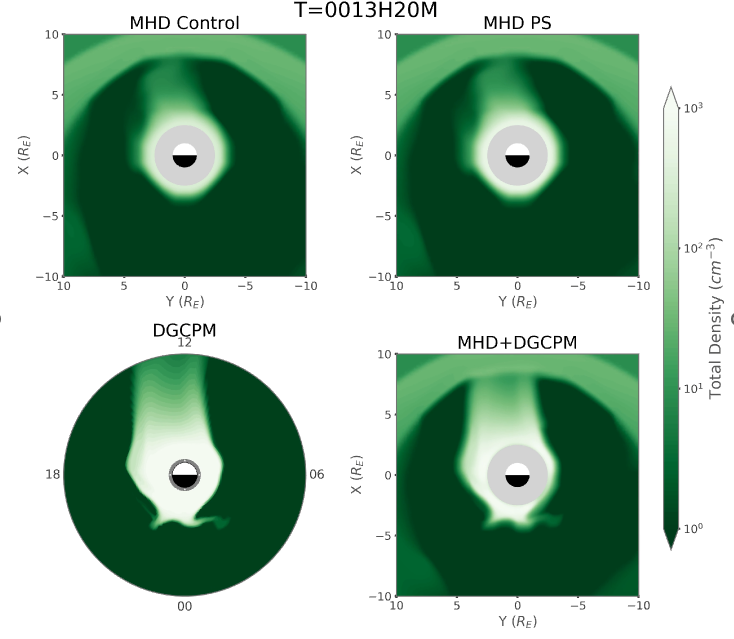
\includegraphics[width=0.5\textwidth]{BATS_DGCPM_coupling.png}
\caption{Affect of coupling on DGPCM and BATS-R-US on realism of plasmasphere in MHD solution} 
\label{fig:METH1}
\end{center}
\end{figure}

\subsubsection{Configuration of RIM}

The Ridley Ionosphere Model (RIM) is a 2-dimensional spherical electric potential solver. For a detailed discussion of how the model works see \citet{Ridley2002}.

In our configuration of the SWMF, RIM is configured to have an ovular polar cap, being driven by provided F10.7 values, and Pederson currents received by coupling with BATS-R-US. For the Simulations presented in this work, the F10.7 values was set to 150.0 cm. Going from BATS-R-US to RIM, coupling takes place at R = 3.5 $R_{E}$ where the Pederson currents are calculated and scaled down to the magnetic field at 120 km altitude, which is where RIM is set to do its own calculations. When passing the Electric field from RIM to BATS-R-US, the coupling occurs at 2.5 $R_{E}$ at which point the electric field calculated by RIM, which is effectively the Dawn-Dusk electric field, is added to the corotation electric field calculated by BATS-R-US \citet{Toth2005}. %I got this information from the SWMF Manuel, should I cite Toth2005 here?

RIM is also coupled to DGCPM, such that the electric field calculated by RIM is used instead of an empirical model such as Tsyganenko 89 or Weber 2000 by DGCPM. The coupling is one way, in which every 10 seconds DGCPM requests electric field data from RIM. The SWMF handles converting the values from RIM's ionosphere grid and internally used units into DGCPM's grid. While both models rely on an ionospheric grid, the grid are not identical and so need to mapped from one to another. SWMF uses a bi-linear interpolation to do this. More information on how the SWMF handles this interpolation can be found in \citet[Toth et al.()]{Toth2005}.

\subsection{Metrics}

The primary value which we will look at is fluence. On the day side of the planet the boundary was a hemispherical shell going from dawn to dusk and spanning $\pm 60^{\circ}$ latitude at 6.6 $R_{E}$, geosynchronous orbit. Fluence is calculated through the surface of the shell as a discrete sum of the flux over the area, 

\begin{equation}
    fluence (\frac{\#}{s}) = \Sigma flux_{r} r^{2} \cos(\theta) d\theta d\phi
    \label{eq:A1}
\end{equation}

where $flux_{r}$ is the radial flux, r is the radius fixed to 4204860000 cm which is 6.6 $R_{E}$ on the dayside, $\theta$ is the latitude, and $\phi$ is the longitude. $d\theta$ and $d\phi$ are the discrete step in theta and phi with values of $\pi/90$ due to the resolution of data points on the spherical shell. The flux is calculated from the density and bulk flow velocities of the fluids taken from BATS-R-US. On the night side the boundary through which we measure flux and calculate fluence is a spherical shell of 10 $R_{E}$ going from dawn to dusk and $\pm 30^{\circ}$ latitude. Figure \ref{fig:RESULT1} shows the fluence of the fluids in BATS-R-US as they pass the measurement boundary. 

\section{Analysis}

\subsection{Ideal Square Wave}

The first simulation done for the study was an idealized square wave event. The solar wind had a constant density and velocity of 5 $/cm^{-3}$ and 450 km/s. The $B_{z}$ component of the interplanetary magnetic field (IMF) began at +5 nT flipping to -10 nT after 8 hours, marking the start of the storm. There was a constant value of $B_{y}  = +2 nT$ which moves the reconnection line slightly out of the equatorial plane. There was no $B_{x}$ tilt. 

\begin{figure}[!ht]
\begin{center}
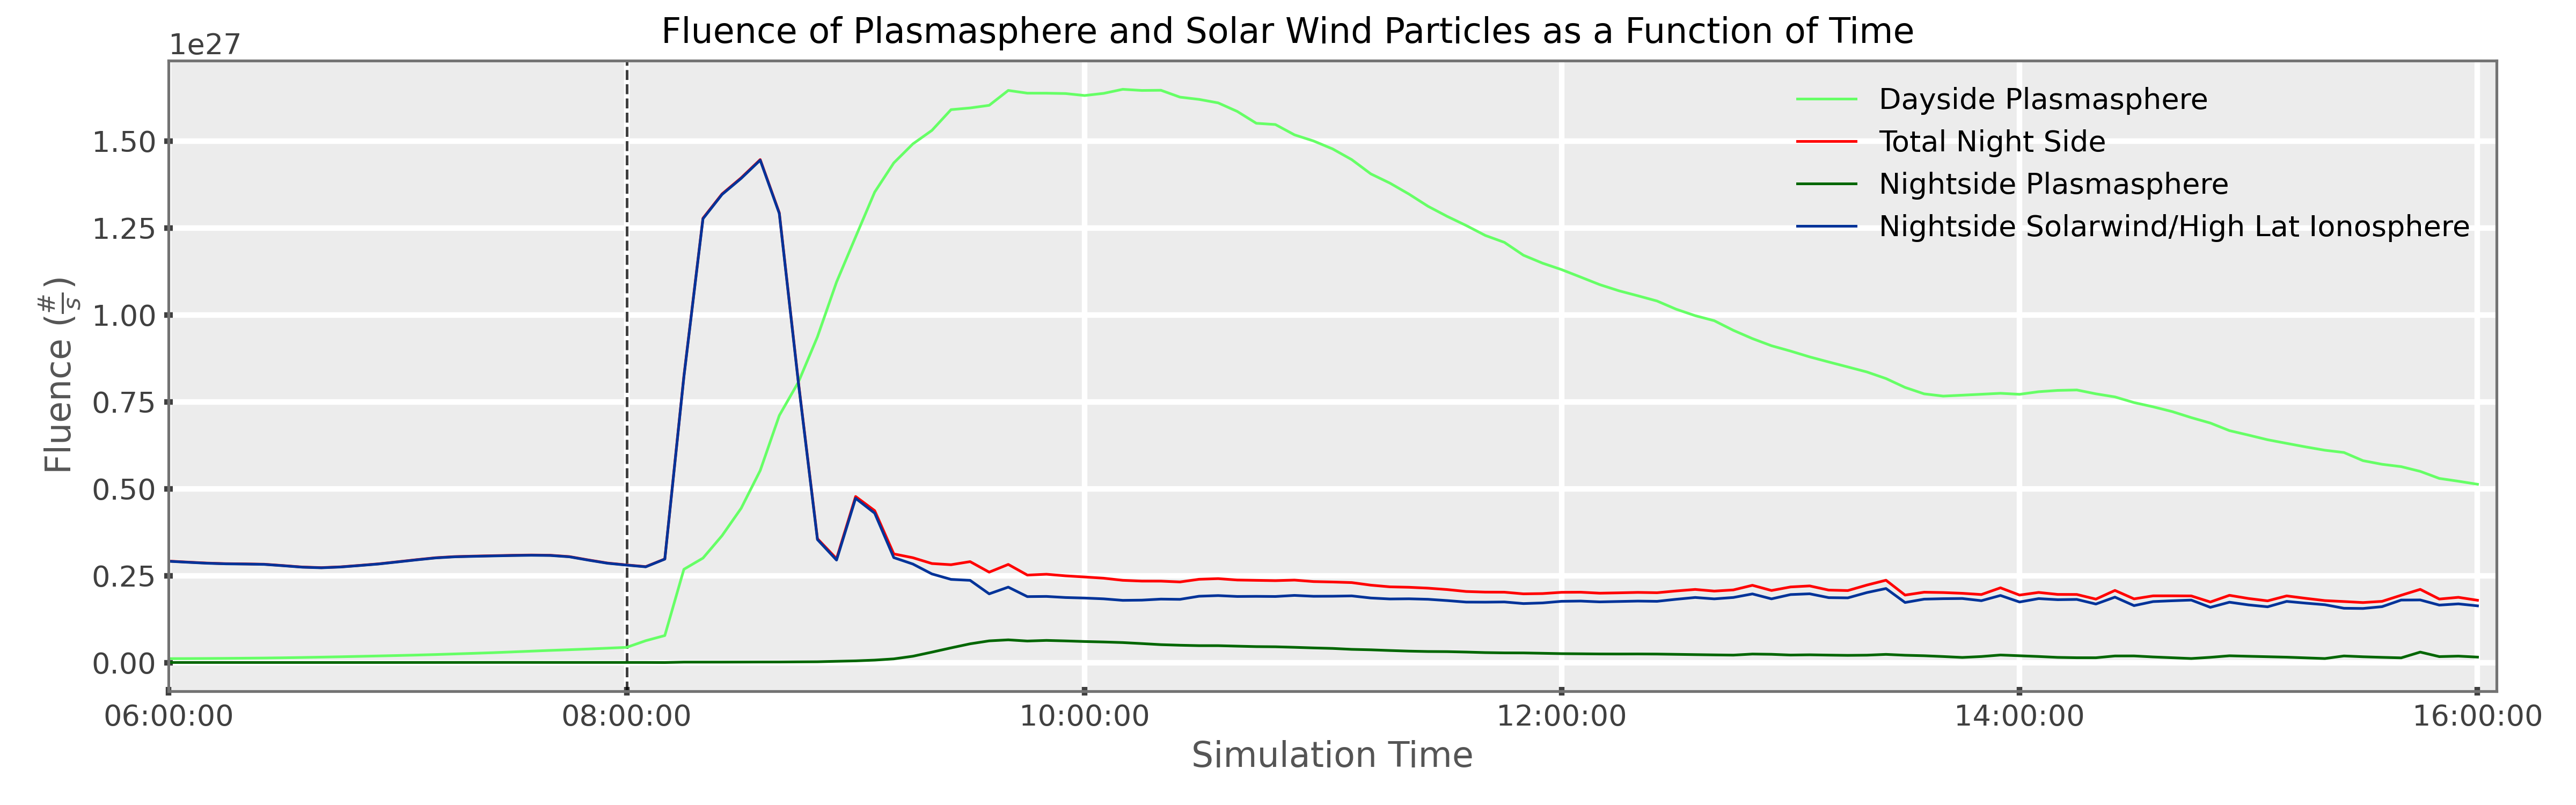
\includegraphics[width=0.9\textwidth]{FluenceAbs_LimCoLat.png}
\caption{Fluence of Plasma Fluids in BATS-R-US across day and night side boundaries.}
\label{fig:RESULT1}
\end{center}
\end{figure}

As we see the plasmasphere flows strongly out the dayside boundary, indicating a strong plume flow. %I could insert a BATS slice showing this. Could add in the measurement circles, make it a bit clearer. 
The value is comparable to ionospheric outflow once the storm begins. By comparing the magnitude of the fluence of plasmasphere material leaving the plasmasphere on the dayside to the fluence of the plasmasphere crossing the night side boundary we see that we lose an order of magnitude of material during the process of recirculation. This indicates that most of the material is lost to the solar wind. The spike in solar wind and high latitude ionosphere fluid crossing the night side boundary is explained by a build up of cold plasma on the night side due to flow patterns, being injected towards the earth as the magnetosphere collapses. After this initial spike we see that the amount of combined solar and polar wind crossing the night side boundary is comparable to that of the plasmasphere material which has recirculated. For a more detailed comparison of the fluid crossing the night side boundary we look to figure \ref{fig:RESULT2}. 

\begin{figure}[!ht]
\begin{center}
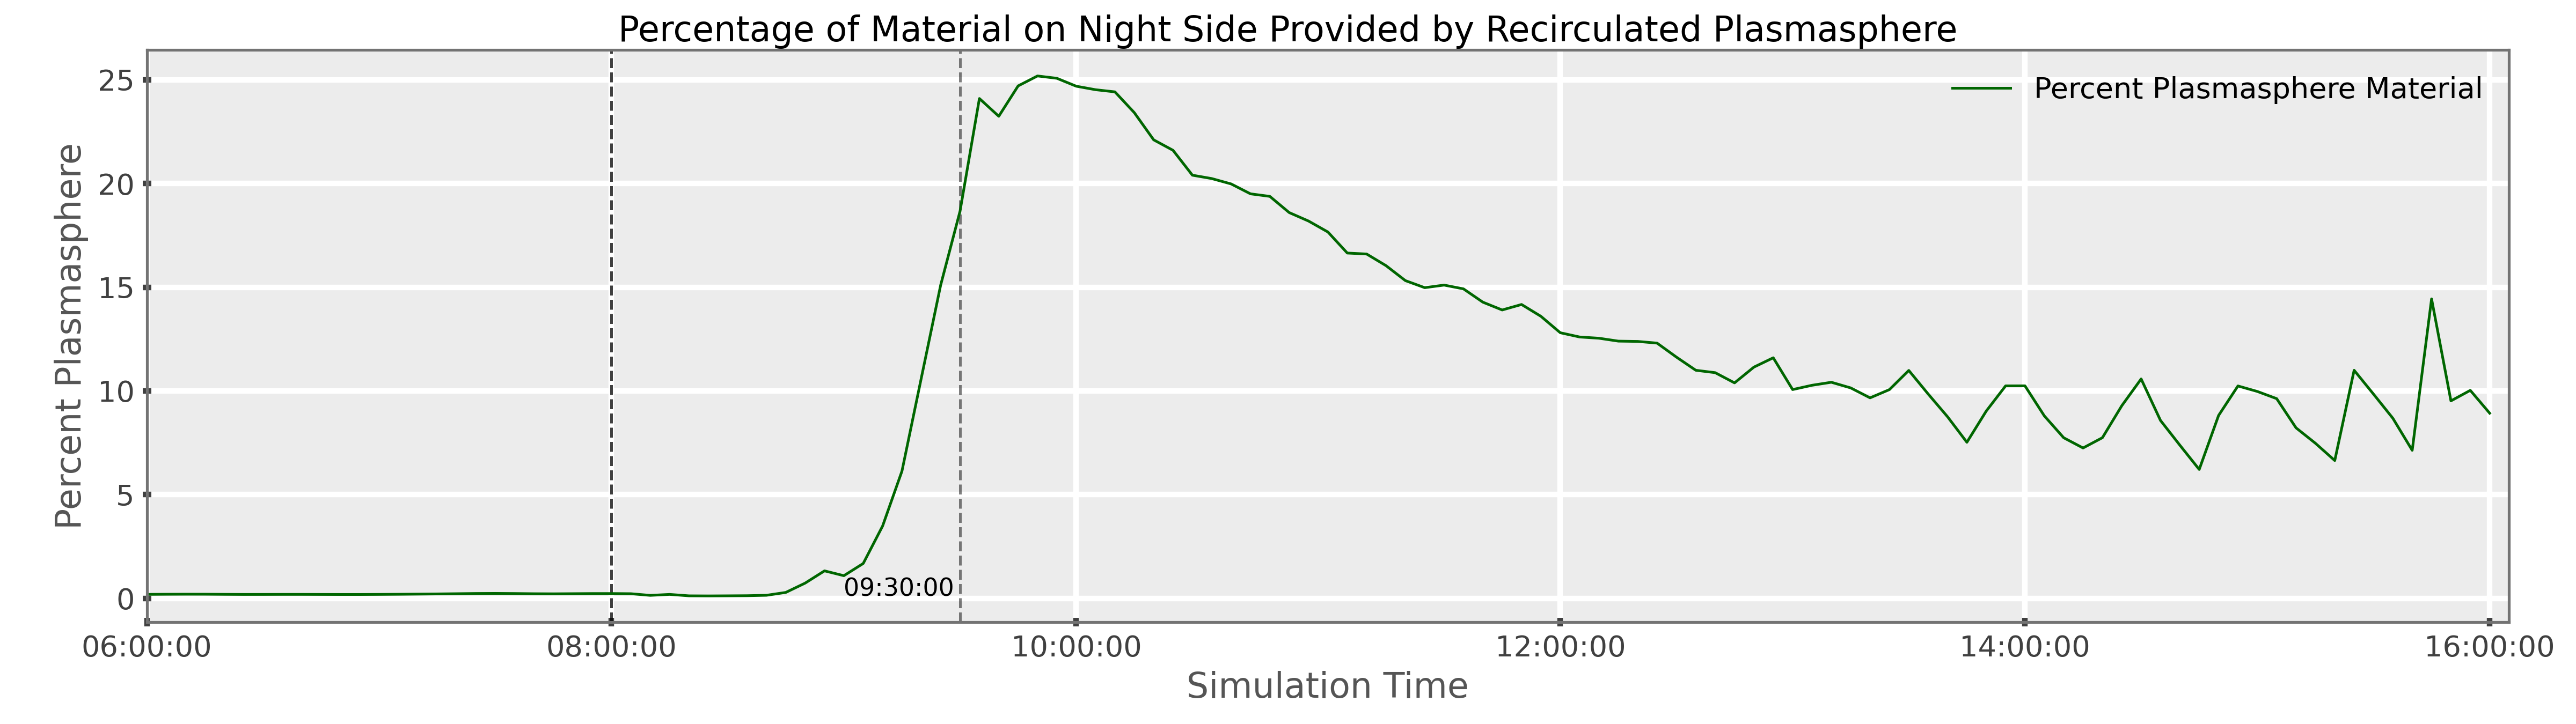
\includegraphics[width=0.9\textwidth]{PrecentPlasNightSide.png}
\caption{Percent Contribution by Recirculated Plasmasphere material of Total Night Side Fluence in Ideal Square Wave Event}
\label{fig:RESULT2}
\end{center}
\end{figure}

Figure \ref{fig:RESULT2} reports what percentage of the material crossing the night side boundary was provided by the recirculated plasmasphere material. We see that there is a delay between storm onset and plasmasphere material having recirculated. Once the dayside plume has vented a substantial amount of material we see that the recaptured portion is still more then 10\% of the total plasma content crossing the night side for three and a half hours. The maximum contribution of the recirculated material was 25\%, with contributions over 20\% lasting about an hour. Figure \ref{fig:REFERENCE1} shows the results of an experiment done in \citet[Welling et al.(2011)]{Welling2011} where $O^{+}$ was injected into the inner magnetosphere in windows centered around dawn, midnight, and dusk. As Figure \ref{fig:REFERENCE1} demonstrates, the more dawn-ward material is injected into the ring current the more likely it is to remain on a closed drift path and contribute to the ring current. 

\begin{figure}
    \centering
    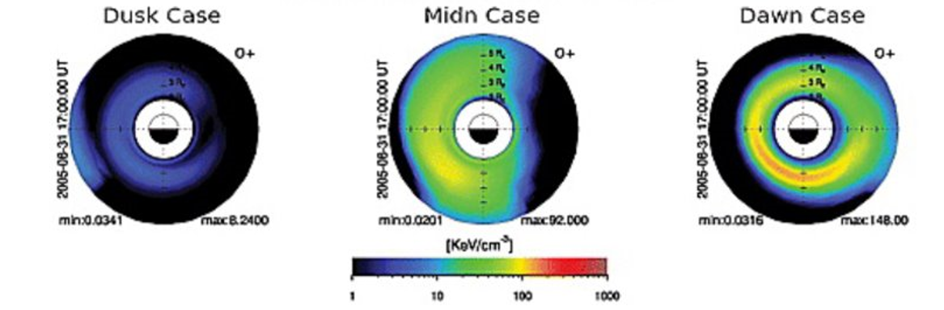
\includegraphics[width=0.7\textwidth]{Welling2011_O_injection.png}
    \caption{$O^{+}$ injections into the ring current adapted from \citet[Welling et al.(2011)]{Welling2011}}
    \label{fig:REFERENCE1}
\end{figure}

A consequence of figure \ref{fig:REFERENCE1} is that in addition to considering the absolute contribution of the fluids in BATS-R-US to the plasma sheet we must also consider where those contributions were made in space. Figure \ref{fig:RESULT4} shows what percentage of the total material contributing to the plasma sheet was provided by the plasmasphere, broken down by magnetic local time. The value reported in figure \ref{fig:RESULT4} is not fluence, as that is calculated over an area. Instead the calculation in eq. \ref{eq:A1} was done only along lines of constant longitude, causing the resulting value to have units of $cm ^{-1} s^{-1}$. What we see here is that, relative to the combined solar wind and polar wind fluid, most of the contribution of the recirculated plasmasphere material is centered in a window spanning midnight to 2 a.m. local time. The QR codes [insert the references once the internet turns back on] show that the flux of the solar wind primarily passed through our measurement boundary in a window centered around 22 LT. The recirculated plasmasphere has a maximum contribution of 70\% the total fluence across the boundary when broken down by MLT. Thus, we can bound the relative contribution of the recirculated plasmasphere material to the plasma sheet to be between 25-70\% depending on the phase of the storm and likely hood of injected plasma remaining on closed drift paths. 

\begin{figure}[!ht]
\begin{center}
    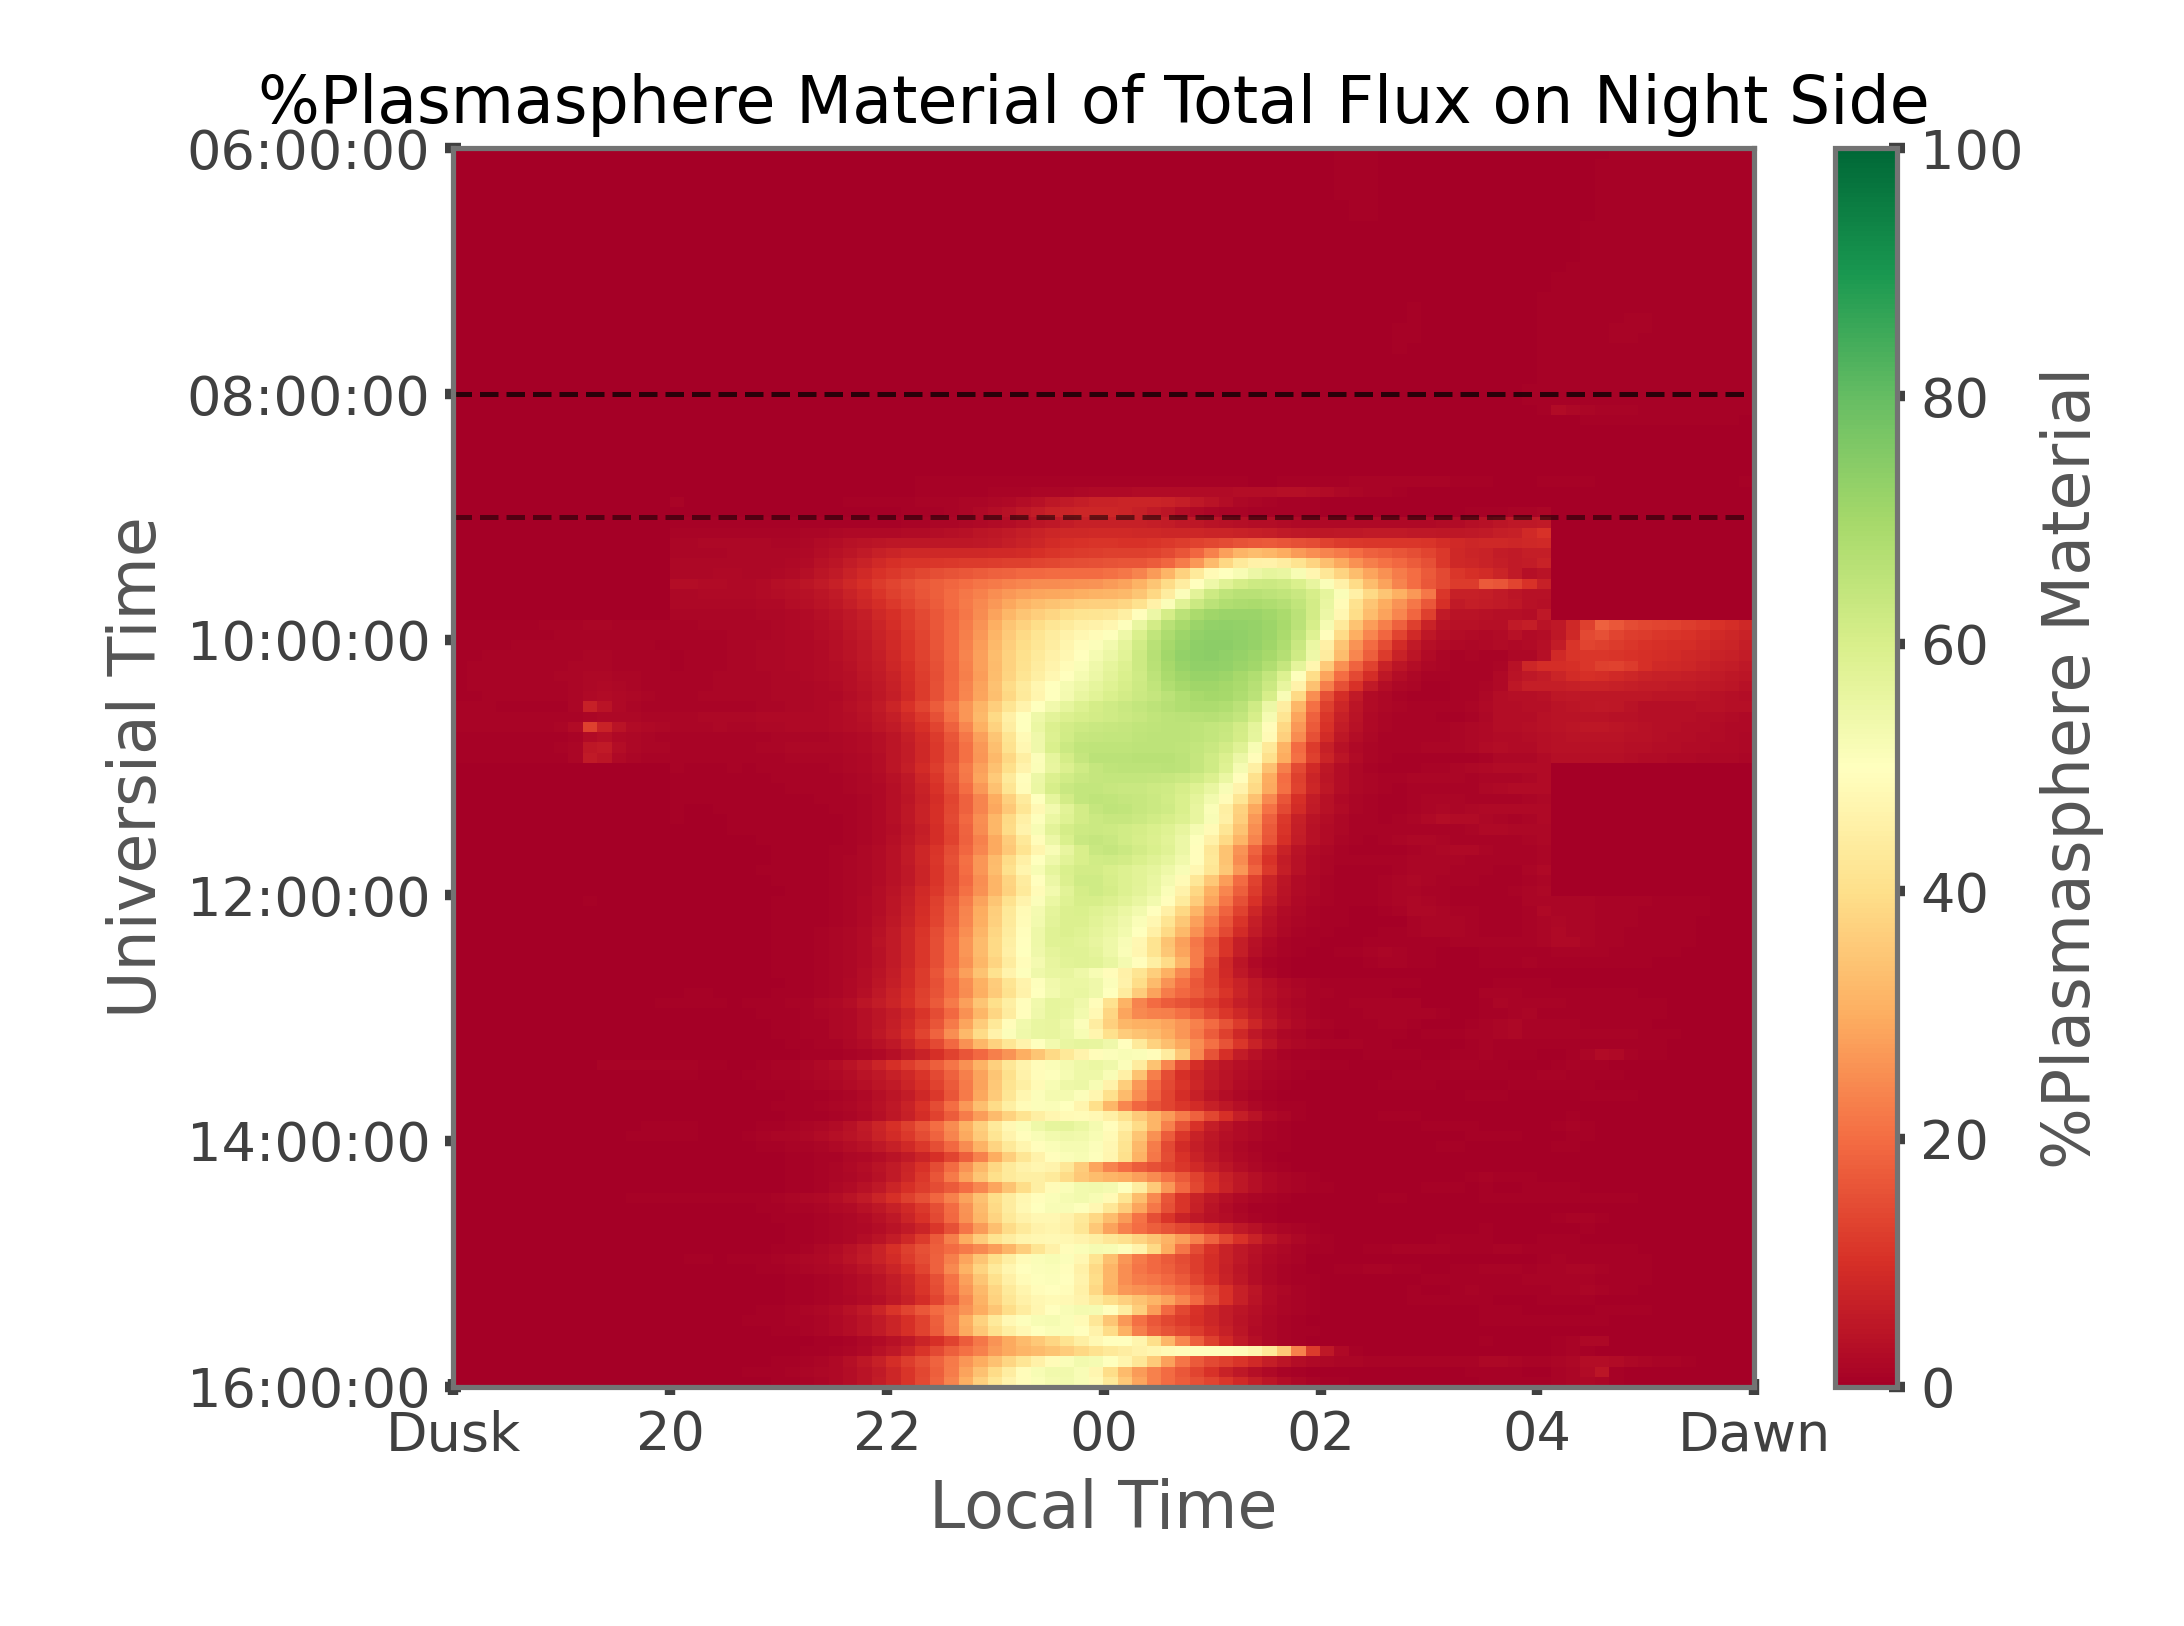
\includegraphics[width=0.7\textwidth]{PCPLonCoLat.png}
    \caption{Percent Contribution of Recirculated Plasmasphere material by Local Time in Ideal Square Wave.}
    \label{fig:RESULT3}
\end{center}
\end{figure}

\subsection{Idealized Corotating Interaction Region}

The second event studied for this paper is an idealized corotating interaction region. The event was constructed by taking a time averaged epoch analysis of 11 storms during solar cycle 23 \citet[Katus et al.(2015)]{Katus2015}. The storm occurs in two phases. The first phase of the storm starts after 6 hours, and begins as a sharp southward turning in the $B_{z}$ component of the magnetic field of about 7.5 nT. At the same time the density of the solar wind increases from an average of 12.5 $/cm^{-3}$ up to 22. 5 $/cm^{-3}$ before recovering to 12.5 $/cm^{-3}$ at the end of the storm. The idealized CIR storm as a long recovery period of 65 hours \citet[Katus et al.(2015)]{Katus2015}. As this study is interested in the main phase of the storm only the first 30 hours of the ideal CIR storm was simulated. The velocity of the solar wind was much slower then that of the other simulations, beginning at 350 $km/s$ and increasing throughout the simulation up to $525 km/s$. Figure \ref{fig:STORM1} shows a detailed plot of the IMF conditions used for this simulation. 

\begin{figure}[!ht]
\begin{center}
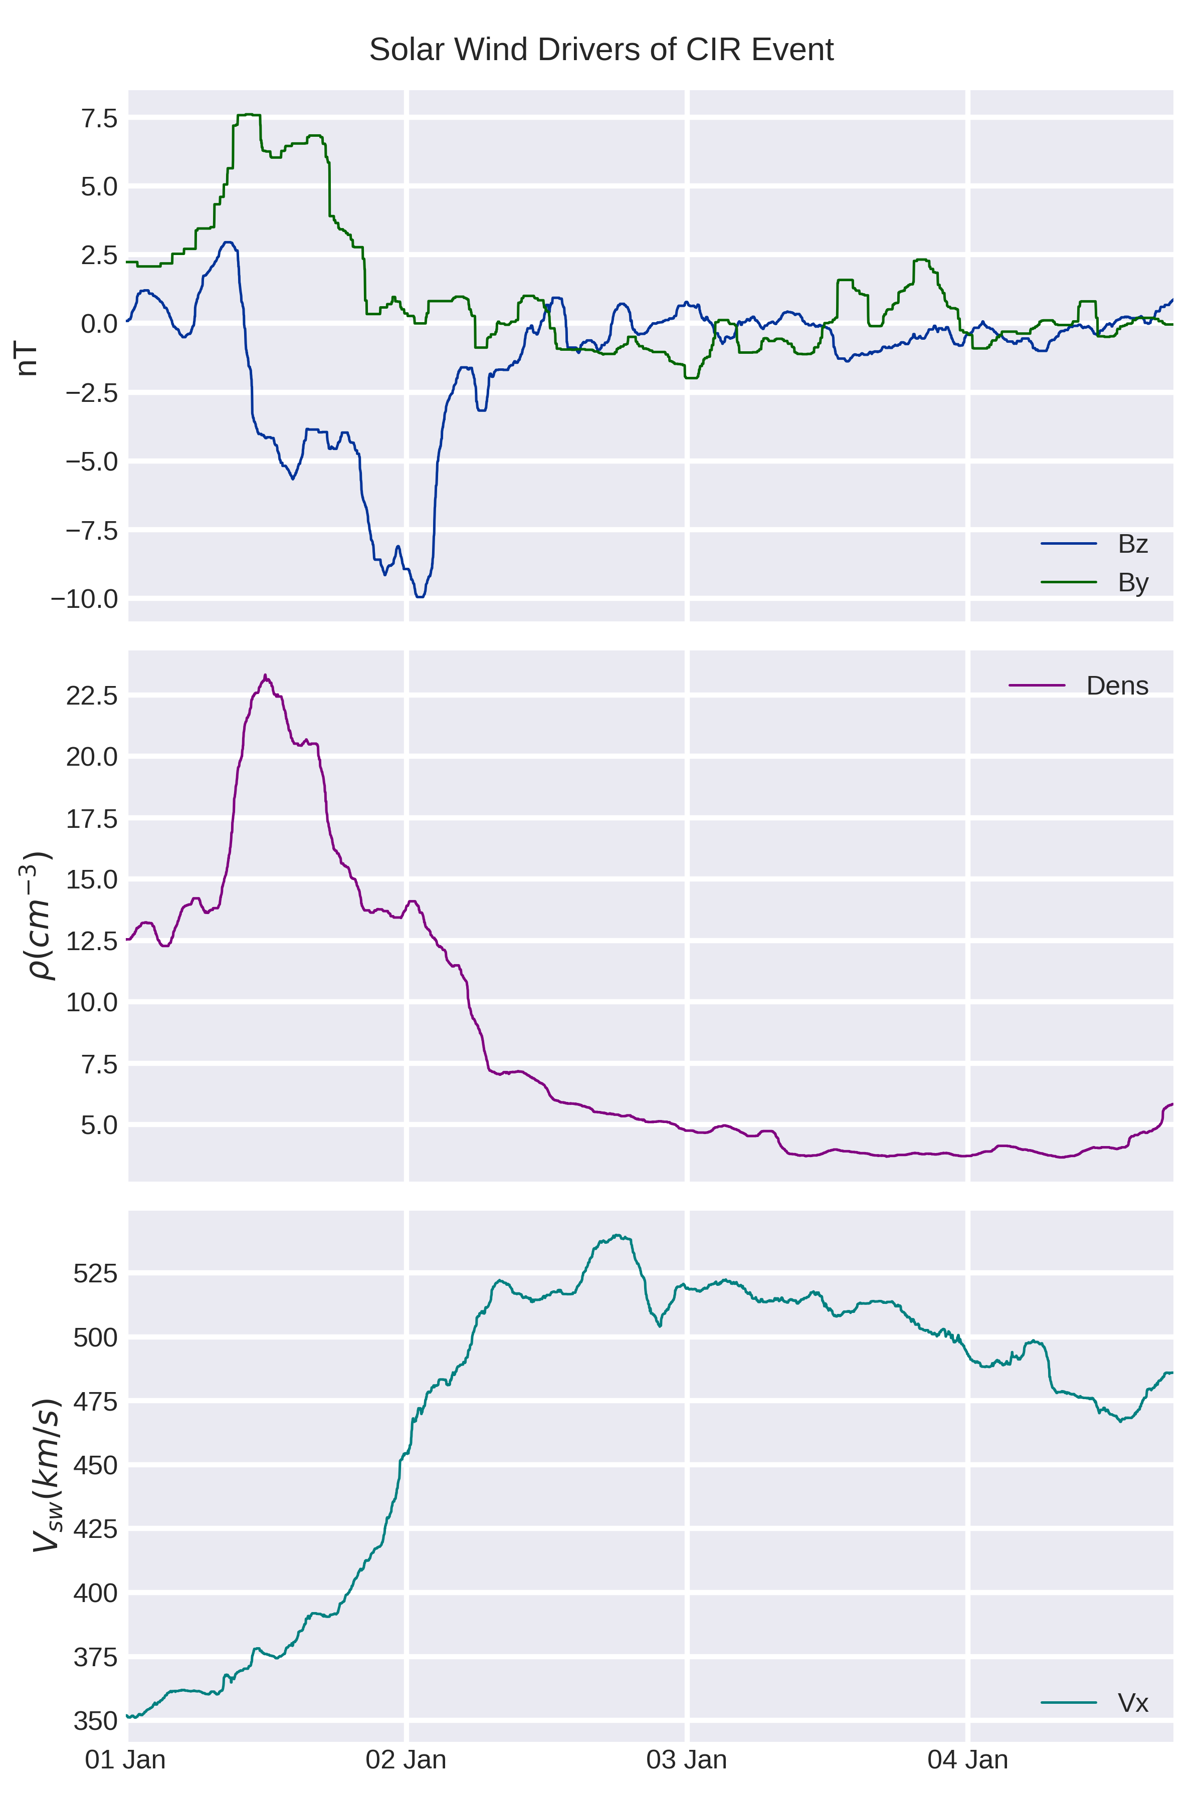
\includegraphics[width=.4\textwidth]{Ideal_CIR.png}
\caption{IMF conditions of Idealized Corotating Interaction Region.}
\label{fig:STORM1}
\end{center}
\end{figure}

Figure \ref{fig:RESULT4} shows the percent contribution of the total fluence crossing the night side boundary that was provided by the recirculated plasmasphere material. We note that the recirculated plasmasphere material began to become a noticeable fraction of the whole much faster than in the ideal square wave event. %Was this plasmasphere leaking like how we saw in CIMI? Seems like it, we do see some of this leaking in the PoC run, but it (qualitatively) is lesser. 
This early increase in the importance of the recirculated plasmasphere contribution is explained by the plasmasphere material leaking out of the plasmasphere and into the tail through the flanks due to viscous interactions, as can be seen in the video included in the supplemental material. The relative contribution is much higher than in the previous event with a maximum contribution of up to 43\%. For a period of four hours soon after the onset of the storm we see that over 20\% over the total material contributing to the plasma sheet is recirculated plasmasphere material. 
 
\begin{figure}[!ht]
\begin{center}
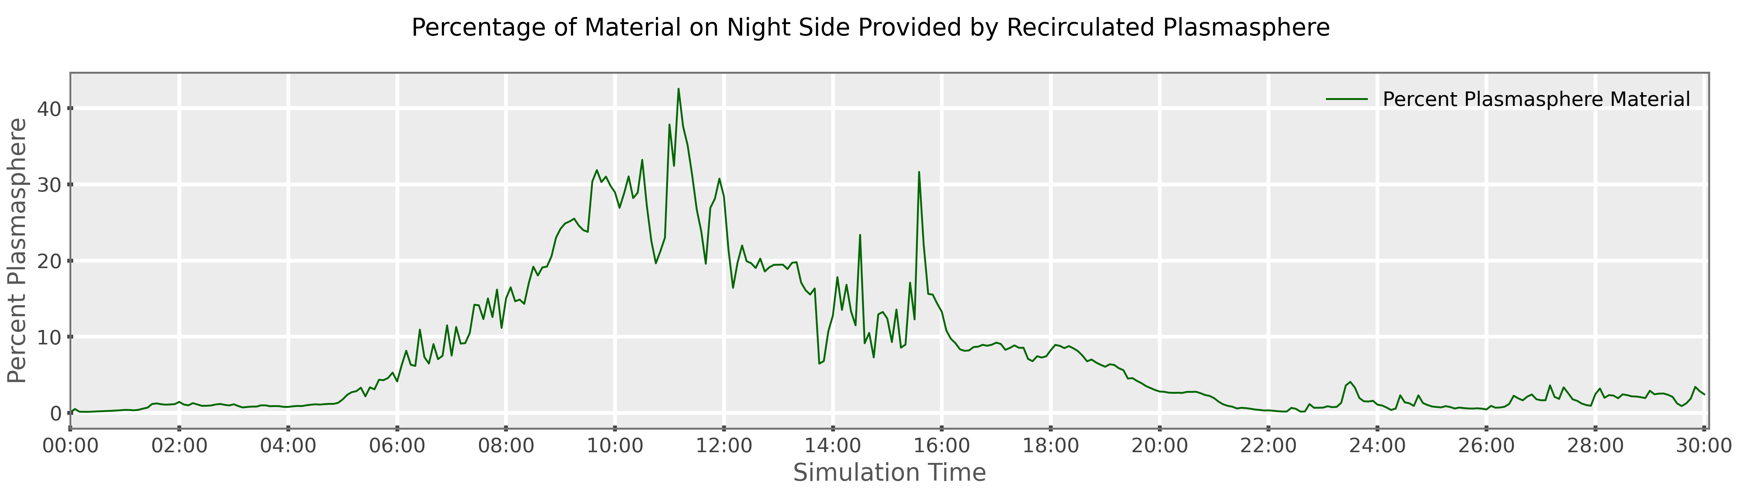
\includegraphics[width=0.9\textwidth]{DGCPM_CIR.PNG}
\caption{Percent Contribution by Recirculated Plasmasphere material of Total Night Side Fluence in Idealized CIR Event}
\label{fig:RESULT4}
\end{center}
\end{figure}

\subsection{Idealized Coronal Mass Ejection - Magnetic Cloud}

the third CME-MC storm:

\begin{figure}[!ht]
\begin{center}
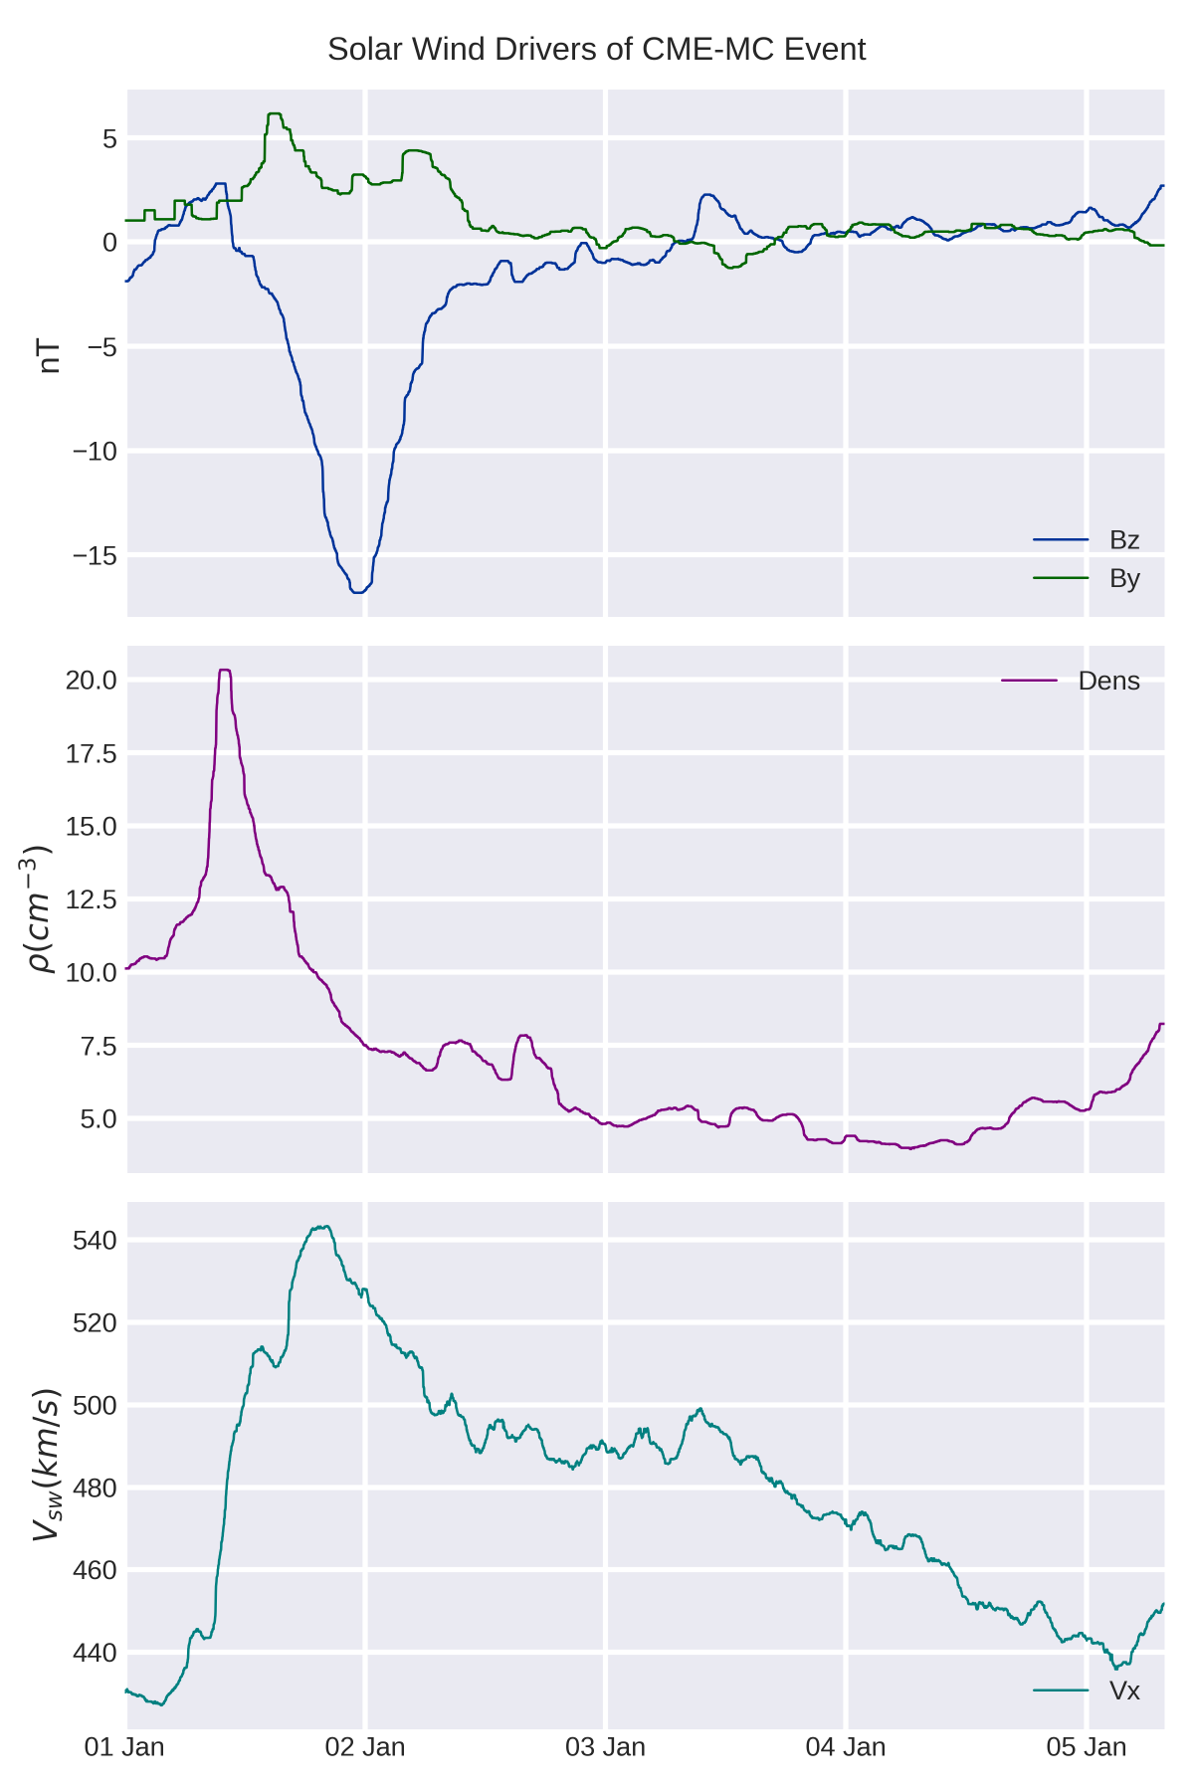
\includegraphics[width=0.4\textwidth]{Ideal Magnetic Cloud.png}
\caption{IMF conditions of Idealized Coronal Mass Ejection - Magnetic Cloud.}
\label{fig:STORM2}
\end{center}
\end{figure}

\subsection{Idealized Coronal Mass Ejection - Sheath Driven}

the fourth CME-SH storm:

\begin{figure}[!ht]
\begin{center}
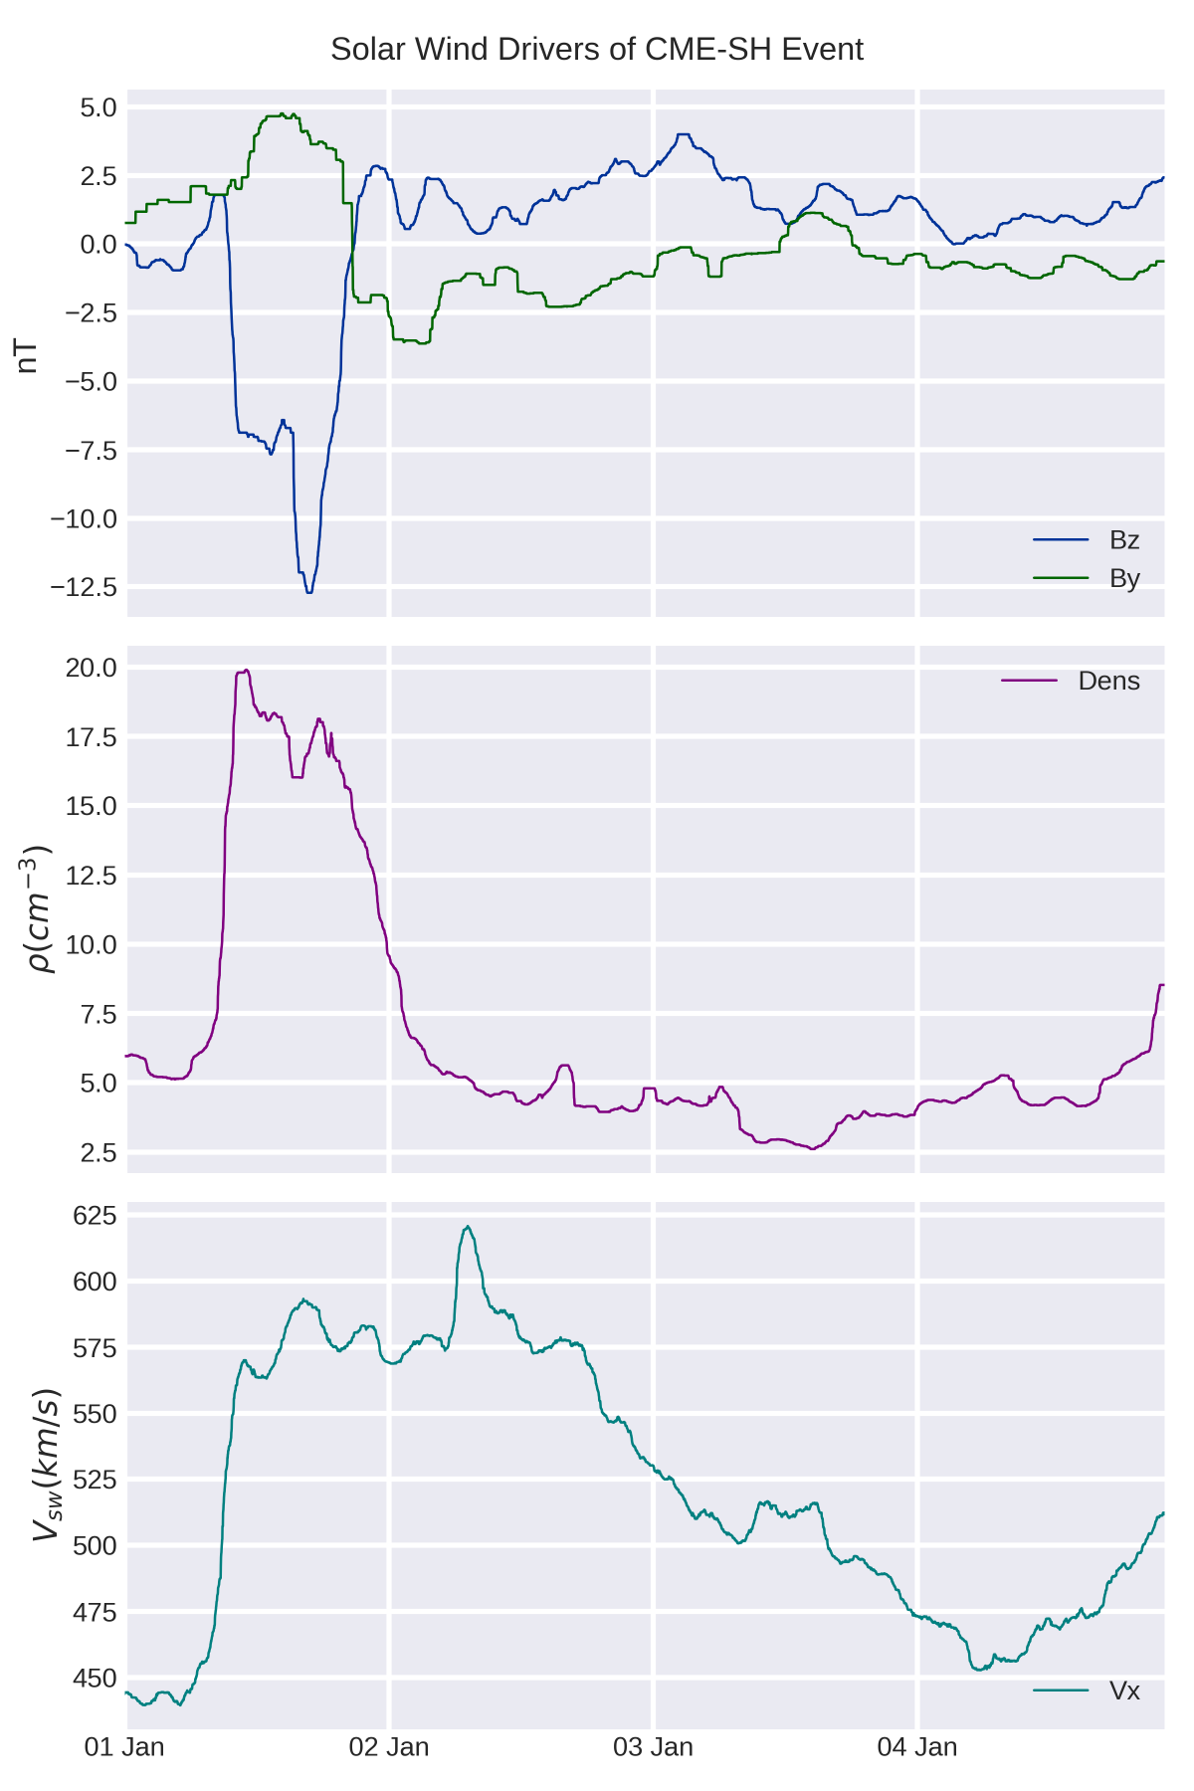
\includegraphics[width=0.4\textwidth]{Ideal_Sheath.png}
\caption{IMF conditions of Idealized Coronal Mass Ejection - Sheath.}
\label{fig:STORM3}
\end{center}
\end{figure}

\section{Discussion}

\section{Conclusion}

\section{Future Work}

Figure \ref{fig:RESULT5} shows how the temperature of the fluids in BATS-R-US evolve as a function of location within the environment. Figure \ref{fig:RESULT5}a shows the absolute temperature difference between the fluids in the noon-midnight meridian plane. We see in the plasma sheet temperature differences of several keV, we see differences of up to 12 keV in the flow outside the equatorial plane near the earth. Figure \ref{fig:RESULT5}b shows the same result but for the equatorial plane. Here we see a much smaller difference between the temperature of the recirculating plasmasphere material and the solar wind material. In the tail, the temperature difference is on the order of several hundred eV. Studying subplots c and d of \ref{fig:RESULT4} we see that the plasmasphere was heated by several hundred eV during the process of recirculation. This difference in temperatures should be detectable by satellite missions such as THEMIS and CLUSTER. 

\begin{figure}[!ht]
\begin{center}
    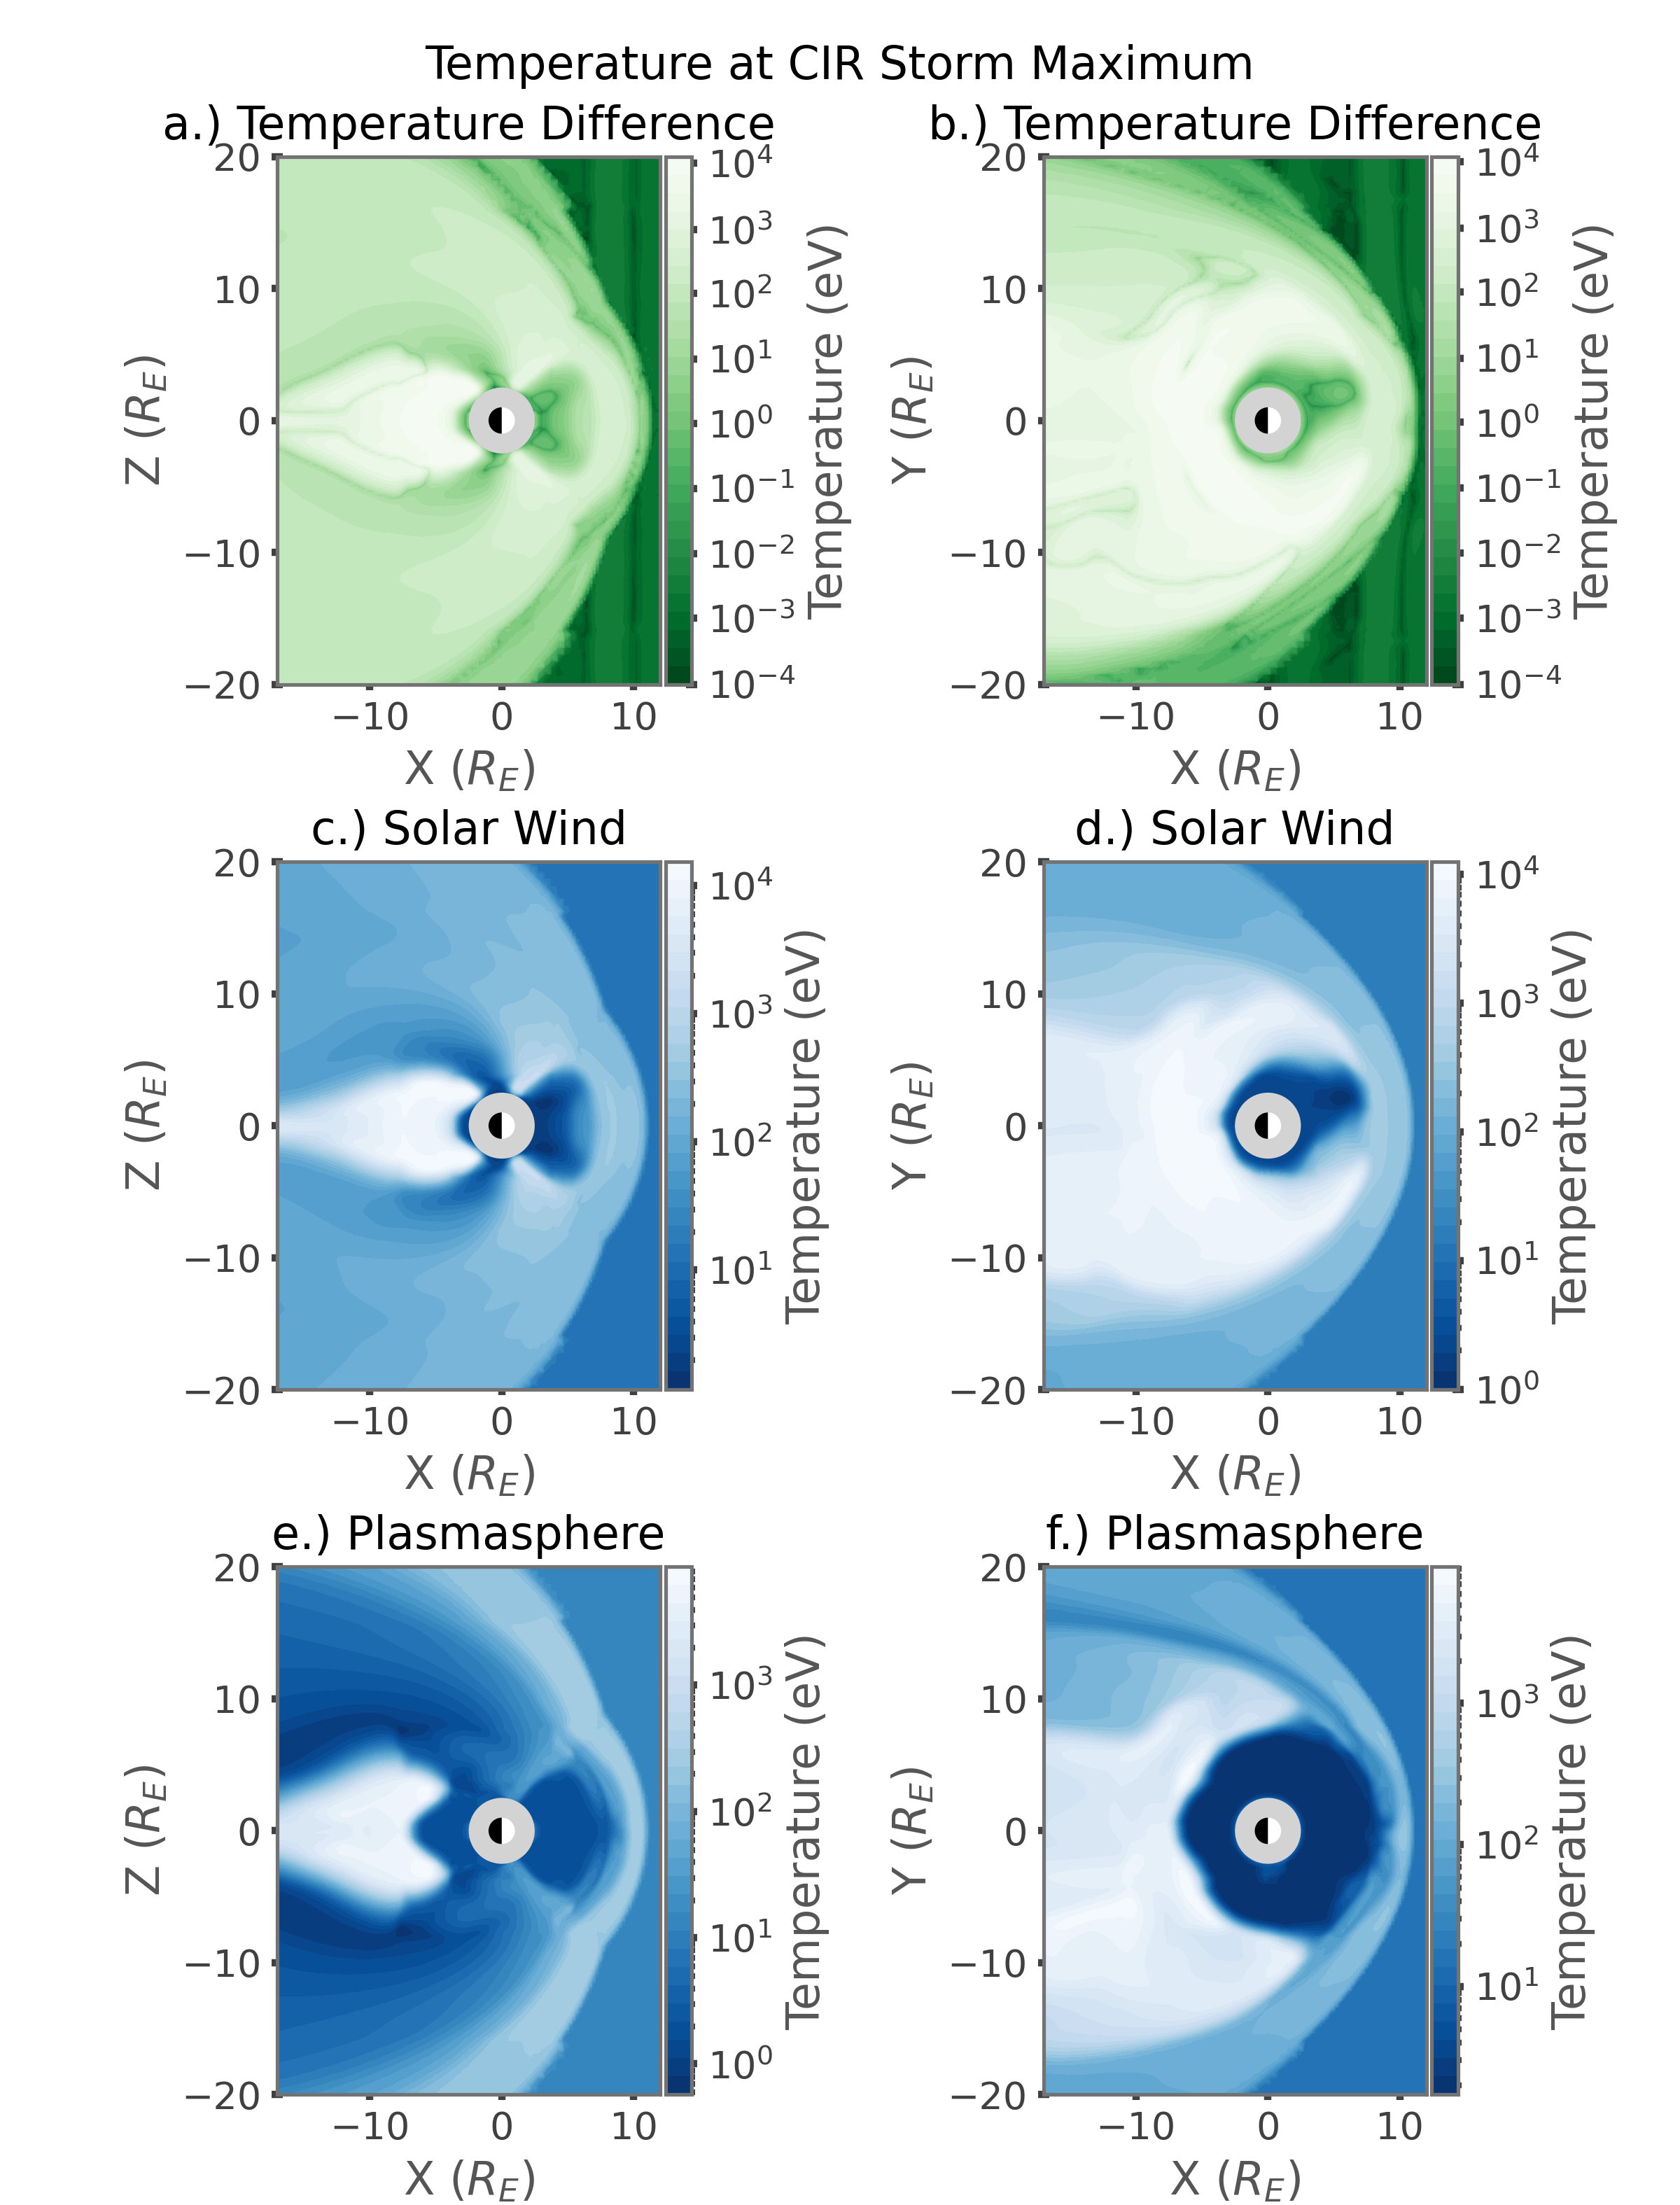
\includegraphics[width=0.7\textwidth]{Temp_Diff_Storm_Maximum.png}
    \caption{Temperature Difference between the fluids in BATS-R-US.}
    \label{fig:RESULT5}
\end{center}
\end{figure}

\section{Acknowledgments}

\section{Funding}



\section{Appendix A} 

Output of the simulations preformed for this paper are to be found at the following repositories: 

1.

2.

3.

4.

Parameter files to reproduce the simulations can be found at the following GitHub repository:

\href{https://github.com/spacecataz/swmf_runfiles.git}{SWMF parameter files}

to change which storm is simulated alter the imf\_*.dat file in the \#UPSTREAM\_INPUT\_FILE command of the GM COMP section of both the PARAM.in.ss and PARAM.in.ta files. 

i.e. change: 

\begin{quote} % a table enviroment could make the formatting look right. But why would I do that?
\#UPSTREAM\_INPUT\_FILE \\
T                          UseUpstreamInputFile \\
imf\_mf\_bzturn\_by.dat    UpstreamFileName \\
0.0                        Satellite\_Y\_Pos \\
0.0                        Satellite\_Z\_Pos \\
\end{quote}

to: 

\begin{quote}
\#UPSTREAM\_INPUT\_FILE \\
T                       UseUpstreamInputFile \\
imf\_cir\_katus.dat     UpstreamFileName \\
0.0                     Satellite\_Y\_Pos \\
0.0                     Satellite\_Z\_Pos \\
\end{quote}

To change from simulating the ideal square wave event to the simulating the idealized CIR event.

The Space Weather Modeling Framework, BATS-R-US, DGCPM, and RIM, as they were configured for this study can be found at:



\section{Abbreviations}
%avoid use of non-standard abbreviations. Do not abbreviations unless used at least four times. Non-standard abbreviations must be defined on first use. 
\begin{itemize}
	\item Space Weather Modeling Framework :: SWMF
	\item Block-Adaptive-Tree-Solar-Roe-Upwind-Scheme :: BATS-R-US
	\item Dynamic Global Core Plasma Model :: DGCPM
	\item Ridely Ionosphere Model :: RIM
	\item Interplanetary Magnetic Field :: IMF
	\item Corotating Interaction Region :: CIR
	\item Coronal Mass Ejection - Magnetic Cloud :: CME-MC
	\item Coronal Mass Ejection - Sheath Driven :: CME-SH
\end{itemize}

\bibliography{RecircPaper}
\bibliographystyle{Frontiers-Vancouver}

\end{document}

% This bibliography style file is intended for texts in ENGLISH
 % This is an author-year citation style bibliography. As such, it is
 % non-standard LaTeX, and requires a special package file to function properly.
 % Such a package is    natbib.sty   by Patrick W. Daly
 % The form of the \bibitem entries is
 %   \bibitem[Jones et al.(1990)]{key}...
 %   \bibitem[Jones et al.(1990)Jones, Baker, and Smith]{key}...
 % The essential feature is that the label (the part in brackets) consists
 % of the author names, as they should appear in the citation, with the year
 % in parentheses following. There must be no space before the opening
 % parenthesis!
 % With natbib v5.3, a full list of authors may also follow the year.
 % In natbib.sty, it is possible to define the type of enclosures that is
 % really wanted (brackets or parentheses), but in either case, there must
 % be parentheses in the label.
 % The \cite command functions as follows:
 %   \citet{key} ==>>                Jones et al. (1990)
 %   \citet*{key} ==>>               Jones, Baker, and Smith (1990)
 %   \citep{key} ==>>                (Jones et al., 1990)
 %   \citep*{key} ==>>               (Jones, Baker, and Smith, 1990)
 %   \citep[chap. 2]{key} ==>>       (Jones et al., 1990, chap. 2)
 %   \citep[e.g.][]{key} ==>>        (e.g. Jones et al., 1990)
 %   \citep[e.g.][p. 32]{key} ==>>   (e.g. Jones et al., 1990, p. 32)
 %   \citeauthor{key} ==>>           Jones et al.
 %   \citeauthor*{key} ==>>          Jones, Baker, and Smith
 %   \citeyear{key} ==>>             1990